\documentclass{beamer}
\usepackage{listings}
\lstset{
%language=C,
frame=single, 
breaklines=true,
columns=fullflexible
}
\usepackage{blkarray}
\usepackage{subcaption}
\usepackage{url}
\usepackage{tikz}
\usepackage{tkz-euclide} % loads  TikZ and tkz-base
%\usetkzobj{all}
\usetikzlibrary{calc,math}
\usepackage{float}
\providecommand{\brak}[1]{\ensuremath{\left(#1\right)}}
\providecommand{\pr}[1]{\ensuremath{\Pr\left(#1\right)}}
\newcommand{\myvec}[1]{\ensuremath{\begin{pmatrix}#1\end{pmatrix}}}
\newcommand\norm[1]{\left\lVert#1\right\rVert}
\renewcommand{\vec}[1]{\mathbf{#1}}
\usepackage[export]{adjustbox}
\usepackage[utf8]{inputenc}
\usepackage{amsmath}
\usepackage{tikz}
\usetikzlibrary{automata, positioning}
\usetheme{Boadilla}

\title{Ramsey 4.2 Tangent and Normal Q.16}
\author{Nelakuditi Rahul Naga - AI20BTECH11029}
\begin{document}

\begin{frame}
\titlepage
\end{frame}

\begin{frame}
\frametitle{Question}
\begin{block}{Ramsey 4.2 Tangent and Normal Q.16}
Find the equations of the circles that touch the lines:
\begin{align}
\myvec{0 & 1}\vec{x} &= 0 \label{eq:1}
\\\myvec{0 & 1}\vec{x} &= 4 \label{eq:2}
\\\myvec{2 & 1}\vec{x} &= 2 \label{eq:3}
\end{align}
\end{block}
\end{frame}

\begin{frame}
\frametitle{Solution}
\begin{block}{General Equation of a Circle}
The general equation of a circle can be expressed as:
\begin{align}
\vec{x^T}\vec{x} + 2\vec{u^T}\vec{x} + f = 0 \label{eq:4}
\end{align}
If $r$ is radius and $\vec{c}$ is the centre of the circle we have:
\begin{align}
f &=\vec{u^T}\vec{u}-r^2  \label{eq:5} \\  
\vec{c} &=-\vec{u}
\end{align}
\end{block}
\end{frame}

\begin{frame}
\frametitle{}
The standard basis vectors in 2D plane are given by:
\begin{align}
\vec{e_{1}} &= \myvec{1 \\ 0}
\\\vec{e_{2}} &= \myvec{0 \\ 1}
\end{align}

We note that the lines \eqref{eq:1} and \eqref{eq:2} are \textbf{parallel} with a common normal along $\vec{e_{2}}$. 

Thus the common normal passing through the centre of the circle is of the form :
\begin{align}
\vec{e_{1}}^T\vec{x} &= k\\
\myvec{1 & 0}\vec{x}&=k 
\end{align}
where $k$ is a constant.
\end{frame}

\begin{frame}
Let the circles of the form \eqref{eq:4} touch the lines \eqref{eq:1} and \eqref{eq:2} at $\vec{M}$ and $\vec{N}$.

$\vec{M}$ is the point of intersection of the following lines:
\begin{align}
\myvec{1 & 0}\vec{x} &=k\\
\myvec{0 & 1}\vec{x} &=0
\end{align}
The above equations can be expressed as the matrix equation :
\begin{align}
\myvec{1 & 0 \\ 0 & 1}\vec{x} = \myvec{k \\ 0}
\end{align}
The augmented matrix for the above equation is given by :
\begin{align}
\myvec{1 & 0 & k\\ 0 & 1 & 0}
\end{align}

As the left part is already a identity matrix ,the intersection point $\vec{M}$ is given by :
\begin{align}
\vec{M} = \myvec{k \\ 0}
\end{align}
\end{frame}

\begin{frame}
\frametitle{}
$\vec{N}$ is the point of intersection of the following lines:
\begin{align}
\myvec{1 & 0}\vec{x} &=k\\
\myvec{0 & 1}\vec{x} &=4
\end{align}
The above equations can be expressed as the matrix equation :
\begin{align}
\myvec{1 & 0 \\ 0 & 1}\vec{x} = \myvec{k \\ 4}
\end{align}
The augmented matrix for the above equation is given by :
\begin{align}
\myvec{1 & 0 & k\\ 0 & 1 & 4}
\end{align}
As the left part is already a identity matrix ,the intersection point $\vec{N}$ is given by :
\begin{align}
\vec{N} = \myvec{k \\ 4}
\end{align}
\end{frame}

\begin{frame}
\frametitle{}
The centre $\vec{c}$ of the circle must be the mid-point of $\vec{M}$ and $\vec{N}$ as $\vec{M}$ and $\vec{N}$ are the touch points of parallel tangents to a circle. Therefore we have:
\begin{align}
\vec{c} &= \dfrac{\myvec{k \\ 0} + \myvec{k \\ 4}}{2}\\
\vec{c} &= \myvec{k \\ 2}
\end{align}
Also the radius $r$ of the circles is given by:
\begin{align}
r &= \dfrac{\norm{\vec{M}-\vec{N}}}{2} \\
r &= \dfrac{\sqrt{(k-k)^{2}+(0-4)^{2}}}{2}\\
r &= 2
\end{align}
\end{frame}

\begin{frame}
\frametitle{}
We have :
\begin{align}
\vec{c} &= \myvec{k \\ 2}
\end{align}
\begin{align}
\implies \vec{u} = -\vec{c} = \myvec{-k \\ -2}
\end{align}
From \eqref{eq:5} we have:
\begin{align}
f &=\myvec{-k&-2}\myvec{-k\\-2}-r^2\\
f &= k^2 + 2^2 -2^2\\
f &= k^2\label{eq:6}
\end{align}
The equation of the remaining line is
\begin{align}
\myvec{2 & 1}\vec{x}& = 2 \label{eq:7}
\end{align}
\end{frame}

\begin{frame}
\frametitle{}
\begin{block}{General equation of a 2nd degree conic and point of contact of the tangent}
The general equation of a second degree can be expressed as :
\begin{align}
\vec{x^T}\vec{V}\vec{x}+2\vec{u^T}\vec{x}+f=0\label{eq:8}
\end{align}
The points of contact $\vec{q}$, of a line with a normal vector $\vec{n}$ to the conics in \eqref{eq:8} are given by:
\begin{align}
\vec{q} = \vec{V}^{-1}\brak{\kappa \vec{n}-\vec{u}} \label{eq:9} \\
\kappa = \pm \sqrt{\frac{\vec{u^T}\vec{V}^{-1}\vec{u}-f}{\vec{n^T}\vec{V}^{-1}\vec{n}}}\label{eq:10}
\end{align}
\end{block}
\end{frame}

\begin{frame}
\frametitle{}
We know that, for a circle, 
\begin{align}
\vec{V} = \vec{I}\label{eq:11}  
\end{align}
and from the properties of an Identity matrix, 
\begin{align}
\vec{I}^{-1} &= \vec{I} \\
\vec{I}\vec{X} &= \vec{X}   
\end{align}
From \eqref{eq:5}, \eqref{eq:7} and \eqref{eq:11} we have:
\begin{align}
\kappa &= \pm \sqrt{\frac{r^2}{\myvec{2 & 1 }\myvec{2 \\ 1 }}} \\
&= \pm \sqrt{\frac{4}{5}} \\
& =  \pm \frac{2}{\sqrt{5}}
\end{align}
\end{frame}

\begin{frame}
\frametitle{}
Therefore from \eqref{eq:9} we have:
\begin{align}
\vec{q} &= \pm \myvec{\dfrac{4}{\sqrt{5}} \\ \dfrac{2}{\sqrt{5}} } - \myvec{-k \\ -2} \\
&=\myvec{\dfrac{\pm 4}{\sqrt{5}} +k \\\dfrac{\pm 2}{\sqrt{5}} +2}
\end{align}
Now $\vec{q}$ lies on the line \eqref{eq:7} therefore,
\begin{align}
\myvec{2 & 1}\myvec{\dfrac{\pm 4}{\sqrt{5}} +k \\\dfrac{\pm 2}{\sqrt{5}} +2} &= 2 \\
\implies k = \pm \sqrt{5}\\
\implies f = k^2 = 5
\end{align}
\end{frame}

\begin{frame}
\frametitle{}
Hence the tangent circles are given by the equations:
\begin{align}
\vec{x^T}\vec{x} + \myvec{2\sqrt{5} & -4}\vec{x} + 5 &= 0 \\
\vec{x^T}\vec{x} + \myvec{-2\sqrt{5} & -4}\vec{x} + 5 &= 0
\end{align}
The illustration of the circles and the lines is shown below :
\begin{figure}[!ht]
       \centering
    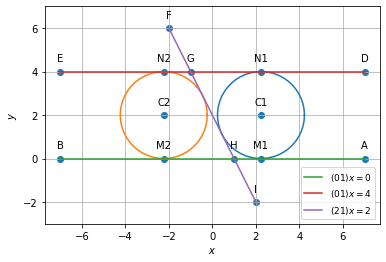
\includegraphics[width=0.6\columnwidth] {Assignment_3_Fig_1.png}
    \caption{Circles touching given lines with centres C1,C2}
    \label{Tangent circles to 3 given lines}
\end{figure}
\end{frame}

\end{document}